\subsection{UC12 - Rimozione del pannello del plug-in dalla dashboard}
\begin{figure}[H]
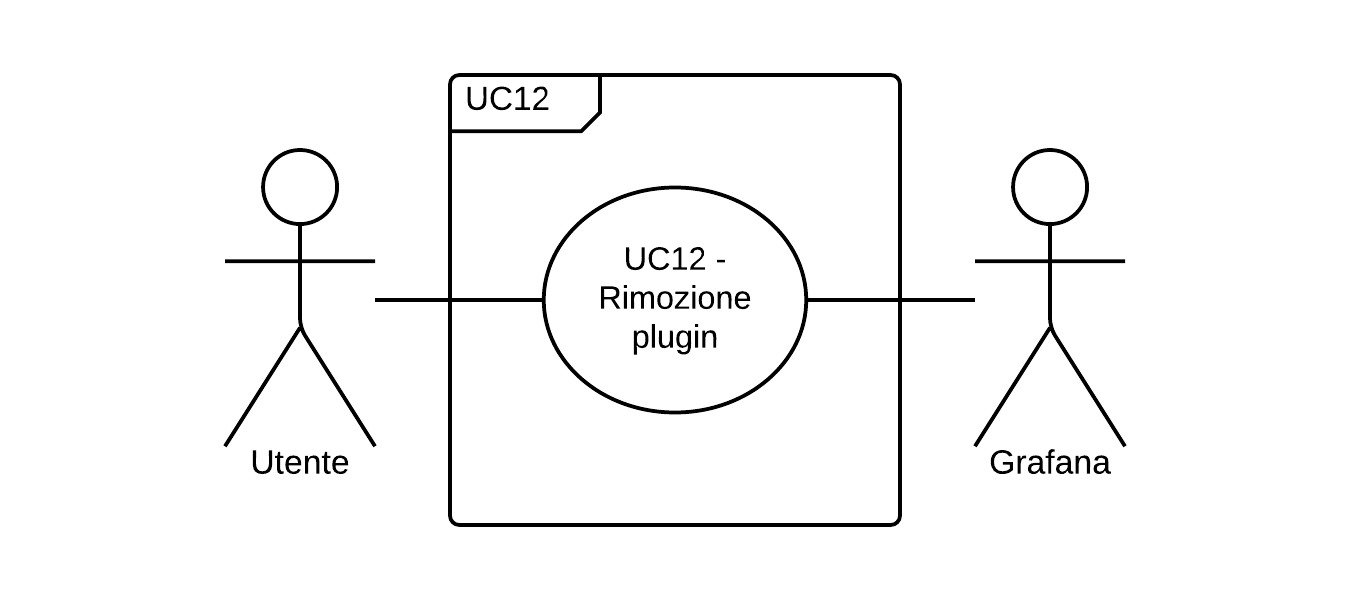
\includegraphics{img/UC12_-_Rimozione_plugin.png}
\caption{Diagramma degli use case di UC12}
\end{figure}
\begin{itemize}
    \item \textbf{Codice identificativo}: UC12;
    \item \textbf{Titolo}: rimozione plug-in;
    \item \textbf{Attori primari}: utente;
    \item \textbf{Attori secondari}: Grafana\glo;
    \item \textbf{Descrizione}: l'utente rimuove il pannello fornito dal plug-in dalla dashboard\glosp di Grafana\glosp in cui era stato inserito, provocandone l'arresto.
    \item \textbf{Precondizioni}: l'utente è autenticato nel sistema software Grafana\glosp e ha avviato il plug-in;
    \item \textbf{Postcondizioni}: l'utente ha rimosso con successo il pannello del plug-in dalla dashboard\glosp di Grafana\glo in cui era stato inserito;
    \item \textbf{Scenario principale}: l'utente utilizzando le funzionalità offerte da Grafana\glosp rimuove il pannello fornito dal plug-in dalla dashboard\glosp di Grafana\glosp in cui era stato inserito, provocandone l'arresto.
\end{itemize}

\subsection{UC20 - Disabilitazione del plug-in}
\begin{figure}[H]
	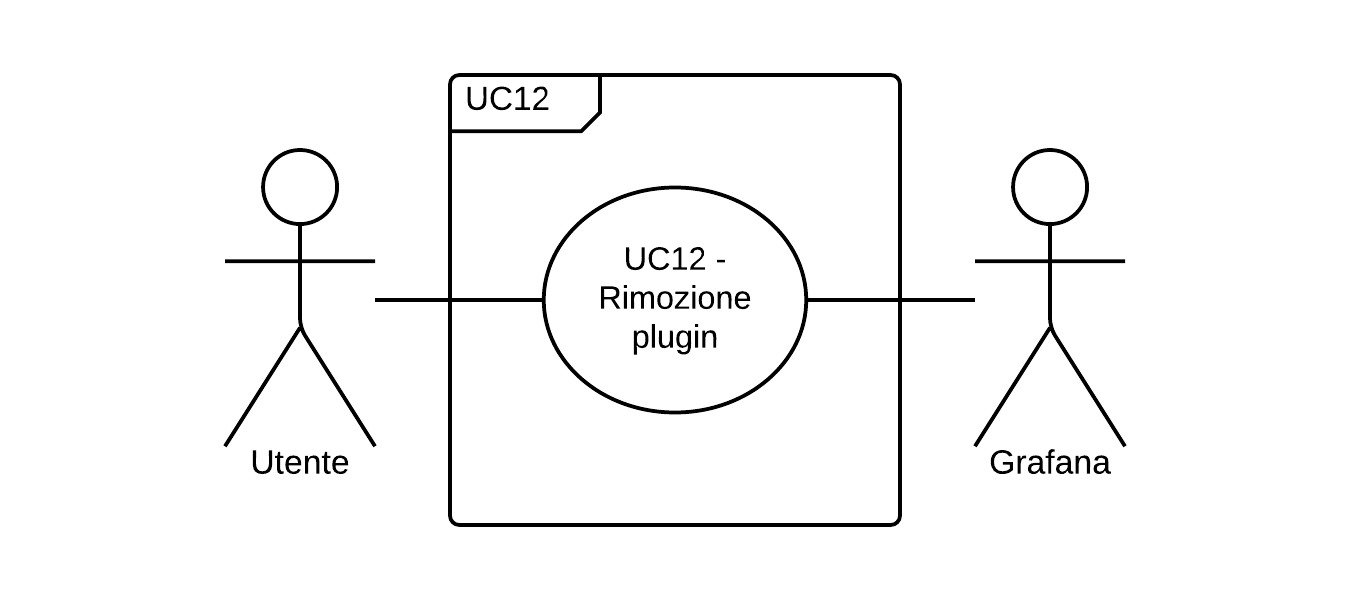
\includegraphics{img/UC12_-_Rimozione_plugin.png}
	\caption{Diagramma degli use case di UC12}
\end{figure}
\begin{itemize}
	\item \textbf{Codice identificativo}: UC20;
	\item \textbf{Titolo}: disabilitazione del plug-in;
	\item \textbf{Attori primari}: utente;
	\item \textbf{Attori secondari}: Grafana\glo;
	\item \textbf{Descrizione}: l'utente esegue l'attività di disabilitazione del plugin dalle impostazioni di Grafana\glo;
	\item \textbf{Precondizioni}: l'utente è autenticato nel sistema software Grafana\glosp e ha abilitato il plug-in;
	\item \textbf{Postcondizioni}: l'utente ha disabilitato con successo il plug-in da Grafana\glo;
	\item \textbf{Scenario principale}: l'utente accede alle impostazioni di Grafana\glosp e disabilita il plug-in.
\end{itemize}